\chapter{Related Work}

Todays use of the internet is heavily based on content dissemination of all kinds of media like audio and video. TV-Shows, clips and tutorials on Youtube, podcasting for educational purposes like on Coursera need to be distributed around the globe. If it is a popular TV-Show the distribution mainly happens within the first few hours of airing. That often leads to a heavy use of bandwith and the bottleneck being the few servers that host that content and their uplinks. In 2008 alone 500 exabytes were created and today's number is a multiple of that [TODO: reference]. That got possible because computers and computing devices became so cheap that almost anybody can afford them. Limited storage on clouds is given free to all users by many providers. When the internet was invented, the situation was a differnet one. There were only a few computers and few resources like tape storage devices, archives or computing power distributed geographically. A client needed some specific information or resources from a specific destination which was known to the client. The client connected through TCP/IP to the Server and after the connection was established and possibly secured the transfer of the information needed by the Client could start. The problem to solve at that time was clearly resource sharing versus today's content dissemination.

TCP/IP is no longer best suited for todays use of the internet. One of the main reasons is that a TCP/IP connection is established between two machines only. Content Dissemination best requires a multipoint to multipoint connection. Another reason is that the Client often does not know where to get some specific information from (and doesn't care) but knows exactly what she wants. Therefore a paradigme shift from host-centric networks started to evolve towards content-centric networks.

\section{Named Data Network / Content Centric Networks}

Named Data Network (NDN) is implemented using the Content Centric Networking (CCN) paradigme. In CCN the content is made directly addressable and routable by name. An Interest (request by a client) is sent out and routed according to it's name until it reaches some endpoint that is able to respond with Content Objects to that Interest. Some of the main goals of CCN is better utilization of the bandwith by increasing throughput and decreasing network traffic, better security, availability, flexibility and scalability of the networks. Better utilization of the bandwith can be achieved by multicasting the same content to several endpoints and not re-unicasting the same content over and over again through the same channels near the content source. Also content caching in intermediate nodes reduces the strain on bandwith and increases overall efficiency. Better security is achieved by hashing and signing the content itself instead the point-to-point connection between two hosts. Encrypting the data leads to more privacy within the internet and can substitute many current access policy patterns used by servers and webpages. Better Availability and flexibility are intrinsically given by content caching. Better scalability is achieved by not needing pre-planned structures like CDN's and P2P networks. Data is not only kept at the content producer but everywhere along the route if necessary.

\begin{figure}[h]
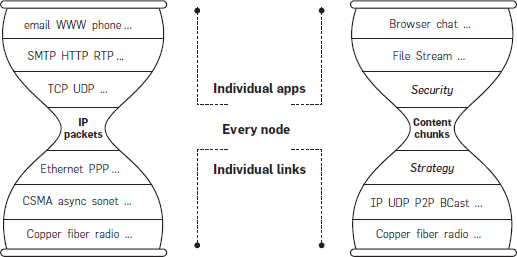
\includegraphics[scale=0.6]{chapter-2/NetworkStack}
\centering
\end{figure}

In Figure 1 the IP and CCN protocol stacks are compared to each other. Both protcol stacks are built in a modular fashion that makes the architecture very flexibl and scalable. The thin waste of the TCP/IP protocol stack consists of IP packages that have a source address and a destination address. This Network Layer is kept very simple and it makes only very weak demands on layer 2. These weak demands on the lower layer make much of the attractivness of IP. This thin waist in TCP/IP protocol stack (\emph{where}) is replaced in CCN with a content layer (\emph{what}) that describes what the package is and has even fewer demands on the lower layer, keeping much of the advantages from IP. Lower layers of the CCN protocol stack are responsible for the routing, encoding and decoding of the information while the higher layers consist of security and the interpretation of the information. Because of the modularity CCN can be implemented on top of IP.

Two big differences of TCP/IP and CNN are the strategy layer and the security layer. The strategy layer is responsible for all dynamic routing decisions based on the name and the strategy. The strategy can be a different one for different namespaces. E.g. an emergency message would be always broadcasted according to it's name. The Security layer differs from the TCP/IP protocal stack since in CCN the content chunks are signed and encrypted instead of securing the connection.

\subsection{CCN/NDN Node Model}

In CCN there are no clients and servers anymore but \textbf{Consumers} and \textbf{Producers}. Consumers request some information by sending out an \textbf{Interest}. This interest packet consists of a content name, some selectors and a nonce. The interest is being forwarded according to the node's strategy it passes until it reaches a node that can satisfy the interest. If a node can satisfy the received interest, it will respond with a \textbf{data} package consisting of the same content name as the interest, a signature, signed info and the data. The data will be be sent back towards the consumer. The node having the requested information is called producer (it generates the data) (TODO:is an intermidiate node that does NOT generate it but supports it also a producer???).

\begin{figure}[h]
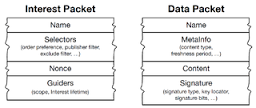
\includegraphics[scale=1]{chapter-2/InterestAndData}
\centering
\end{figure}

The most important tables for routing the interest to the producer and the data back to the consumer are called pending interest table (PIT), forwarding information base (FIB), and the content store (CS). They will be explained in the follwing subchapters.

\subsubsection{PIT}

\subsubsection{FIB}

\subsubsection{CS} 


\subsection{Transport and Routing}

\subsection{Content-Based Security}



\section{VANETS}
